\documentclass{standalone}

\usepackage{import}
\subimport{../../../}{preamble.tex}

\usepackage{pgfplots}
\usetikzlibrary{calc, fillbetween}
\pgfplotsset{compat=newest}

\begin{document}

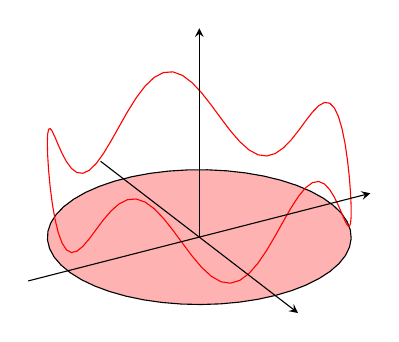
\begin{tikzpicture}
  \begin{axis}[
    view={60}{40},
    axis lines=center,
    axis on top,
    xmin=-1.3,
    xmax=1.3,
    ymin=-1.3,
    ymax=1.3,
    zmin=0,
    zmax=1.05,
    ytick={0},
    ztick={0},
    xtick={0},
    clip=true
    ]
    
    \addplot3 [name=A, fill=red!30, style=densely dotted, no markers, domain=0:360, samples=50, variable=\t] ({cos(\t)},{sin(\t)},{0})--cycle;

    

    \addplot3+ [no markers, domain=0:360, samples=100, variable=\t] ({cos(\t)},{sin(\t)},{0.2*sin(5*\t)+0.3});

    
  \end{axis}
\end{tikzpicture}

\end{document}
%%% Local Variables:
%%% mode: latex
%%% TeX-master: t
%%% End:
